\chapter{Results and Analysis}
\label{chap:4}

%-----------------------------------------------------------------------
%Chapter 4 Findings and Results
%-----------------------------------------------------------------------

% Nomenclature for Chapter 4

% Acronyms for Chapter 4
%	\newacronym{psd}{PSD}{Power Spectral Density}
%	\newacronym{fea}{FEA}{Finite Element Analysis}
%	\newacronym{vf}{VF}{Volume Fraction}
%	\newacronym{naca}{NACA}{National Aviation Commission Advisory}
%	\newacronym{fem}{FEM}{Finite Element Model}
%	\newacronym{leo}{LEO}{Low-Earth Orbit}

%-----------------------------------------------------------------------
\section{Chapter Overview}
%-----------------------------------------------------------------------



\begin{equation}
\label{e:Drag_Force}
F_{d}=\frac{1}{2}C_{d}A\rho v^2
\end{equation}
\nomenclature{$C_{d}$}{Coefficient of drag}
\nomenclature{$A$}{Area of solar panel}
\nomenclature{$\rho$}{Atmospheric density}
\nomenclature{$v$}{Speed of the satellite}

where $C_{d}$ is the drag coefficient, A is the area of solar panel projected in the velocity direction, $\rho$ is the atmospheric density, and $v$ is the speed of the satellite. For a simple approximation it is safe to assume an exponential model for atmospheric density shown in Equation \ref{e:atm}, and a circular orbit which yields Equation \ref{e:Orbital_Vel}:

\begin{equation}
\label{e:atm}
\rho=\rho_o e^{-h/H}
\end{equation}
\nomenclature{$\rho_o$}{Atmospheric density at sea level}
\nomenclature{$h$}{Orbital altitude}
\nomenclature{$H$}{Atmospheric scale height}

\begin{equation}
\label{e:Orbital_Vel}
v=\sqrt[]{\frac{\mu}{r}}
\end{equation}
\nomenclature{$\mu$}{Earth's gravitational parameter}
\nomenclature{$r$}{Orbital radius}

where $\rho_o$ is the representative atmospheric density at sea level, $h$ is the orbital altitude, and $H$ is the Atmospheric Scale Height, which ranges from 6 km to 8 km, and for the purposes of a realistic approximation, 7 km was chosen. In Equation \ref{e:Orbital_Vel}, $v$ is orbital speed, $\mu$ is Earth's Gravitational Parameter, and $r$ is the orbital radius, which is Earth's radius plus the orbital altitude \cite{wiesel2010spaceflight}.

Picking a representative orbital altitude of $r=500$ km, and using constant values of $\mu=398\:601$ km$^3$/s$^2$ and $\rho_o=1.225$ kg/m$^3$, the air density at altitude 
%-----------------------------------------------------------------------
\subsection{1U Demonstration}
\begin{figure}[ht]
	\centering
 	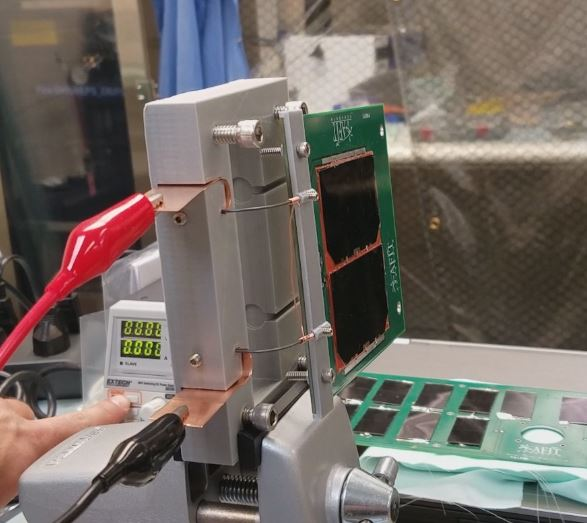
\includegraphics[width=0.305\linewidth]{Ch4/Figures/1U_Demo_1.jpg}
    \caption{Successful 1U demonstration of the Nitinol hinge prototype actuation}
	\label{f:1U_Demo}
\end{figure}
\FloatBarrier
%-----------------------------------------------------------------------


